\documentclass[12pt]{article}
\usepackage[T2A]{fontenc}
\usepackage[utf8]{inputenc}
\usepackage{multirow}
\usepackage{caption}
\usepackage{subcaption}
\usepackage{amsmath}
\usepackage{changepage}
\usepackage{graphicx}
\usepackage{float}
\usepackage[english,russian]{babel}
\usepackage{amsmath, amsfonts, amssymb, amsthm, mathtools}
\usepackage{xcolor}
\usepackage{array}
\usepackage{hyperref}
\usepackage[top = 1.5cm, left = 1.5 cm, right = 1.5 cm, bottom = 3 cm]{geometry}
\graphicspath{ {./images/} }
 
\title{Определение момента инерции тел с использованием трифилярного подвеса}
\author{Шахматов Андрей, Б02-304}
\date{\today}
  
\begin{document}
\begin{titlepage}
    \begin{center}
        {\large МОСКОВСКИЙ ФИЗИКО-ТЕХНИЧЕСКИЙ ИНСТИТУТ (НАЦИОНАЛЬНЫЙ ИССЛЕДОВАТЕЛЬСКИЙ УНИВЕРСИТЕТ)}
    \end{center}
    \begin{center}
        {\large Физтех-школа физики и исследований им. Ландау}
    \end{center}
    
    
    \vspace{3cm}
    {\huge
        \begin{center}
            \textbf{Определение момента инерции тел с использованием трифилярного подвеса}
        \end{center}
    }
    \vspace{2cm}
    \begin{flushright}
        {\LARGE Автор:\\ Шахматов Андрей Юрьевич \\
            \vspace{0.2cm}
            Б02-304}
    \end{flushright}
    \vspace{7 cm}
    \begin{center}
        Долгопрудный 2023
    \end{center}
\end{titlepage}

% \maketitle

\begin{abstract}
    При помощи трифилярного подвеса измерены моменты инерции нескольких тел. Теоретически рассчитаны моменты инерции данных тел. 
    Оценены погрешности полученных моментов инерции и проведен сравнительный анализ теоретически рассчитанных моментов инерции с 
    моментами инерции, рассчитаными экспериментально, в результате которого определено, что с использованием метода расчёта момента инерции тела
    при помощи трифилярного подвеса возможно добиться точности измерения, сравнимой с теоретической.
\end{abstract}

\tableofcontents

\section{Введение}
Измерение момента инерции тела является фундаментальной задачей в механике и имеет важное значение в различных областях науки и техники. 
Однако теоретический расчёт моментов инерции часто бывает слишком сложен из-за формы тела или большого количества составных деталей. 
Потому важной задачей является нахождение экспериментального метода расчёта момента инерции тела с точностью, сравнимой с 
теоретической. Одним из таких методов является расчёт момента инерции с помощью трифилярного подвеса. Цель данной работы заключалась в 
проверке корректности метода определения момента инерции с использованием трифилярного подвеса путём расчёта погрешности измерения и 
сравнения полученного результата с теоретическим.

\section{Методика}
\subsection{Период колебаний груза на трифилярном подвесе}
В эксперименте использовался трифилярный подвес, изображённый на рисунке \ref{fig:1}. Из теории\cite{LabBook} известно, что при условии отсутствия
трения в системе справедливо уравнение малых колебаний:
\begin{equation}\label{eq:1}
    I\ddot{\phi} + mg\frac{Rr}{z_0}\phi = 0
\end{equation}
Где $I$ - момент инерции подвеса, $m$ - масса подвеса, $R, r, z_0$ - геометрические размеры трифилярного подвеса(Рис. \ref{fig:1}).
\begin{figure}
    \begin{center}
        \includegraphics[width=0.5\textwidth]{im.png}
    \end{center}
    \caption{Схема трифилярного подвеса, использованного в эксперименте.}
    \label{fig:1}
\end{figure}
Тогда при малом отклонении системы из положения равновесия возникнут гармонические колебания с периодом $T$:
\begin{equation}\label{eq:2}
    T = 2\pi\sqrt{\frac{Iz_0}{mgRr}}
\end{equation}
Из выражения \ref{eq:2} можно выразить момент инерции подвеса $I$ через массу подвеса $m$, период малых колебаний $T$ и геометрический параметр 
системы $k = \frac{gRr}{4\pi^2z_0}$:
\begin{equation}\label{eq:3}
    I = kmT^2
\end{equation}
С использованием выражения \ref{eq:3} возможно найти момент инерции произвольного тела относительно центра его центра масс. Однако полученное
выражение справедливо только при малой амплитуде колебаний и небольшими потерями энергии, то есть $\tau \gg T$, где $\tau$ - характерное время
затухания колебаний.
\subsection{Нахождение моментов инерции произвольных тел, с использованием трифилярного подвеса}
Для проверки корректности метода нахождения момента инерции с использованием трифилярного подвеса рассмотрены несколько тел с теоретически 
рассчитанными моментами инерции (Прил. \ref{app_1}): полый циллиндр $I_1$ (Рис. \ref{fig:2}), циллиндрическая крышка $I_2$ (Рис. \ref{fig:3}), 
а также два полуциллиндровых груза $I_3$. 
\begin{figure}
    \begin{center}
        \includegraphics[width=0.3\textwidth]{body1.png}
    \end{center}
    \caption{Схема полого циллиндра, использованного в экспперименте.}
    \label{fig:2}
\end{figure}
\begin{figure}
    \begin{center}
        \includegraphics[width=0.3\textwidth]{body3.png}
    \end{center}
    \caption{Схема циллиндрической крышки, использованной в экспперименте.}
    \label{fig:3}
\end{figure}
Для нахождения момента инерции относительно центра масс ($I_1$ и $I_2$) следует разместить груз на трифилярном подвесе таким образом, чтобы
центра масс груза и подвеса совпадали. Тогда возможно найти момент инерции всей системы как сумму моментом $I_1$ и $I_0$, $I_0$ - момент инерции
трифилярного подвеса.
При наличии двух тел ($I_3$) возможно увеличить точность измерения момента инерции, разположив два тела на трифилярном подвесе так, чтобы центр масс двух 
тел совпадал с центром масс трифилярного подвеса. Используя закон Гюйгенса-Штейнера, получено выражение для измеренного момента инерции всей 
системы $I$, где $m$ - масса одного груза, $d$ - расстояние от оси момента инерции до центра масс системы, $m_0$ - масса трифилярного подвеса:
\begin{equation}\label{eq:4}
    k(2m + m_0)T^2 = I = I_0 + 2(I_3 + md^2)
\end{equation}
В выражении \ref{eq:4} получена линейная свзяь $T^2$ и $d^2$, потому возможно построить график линейной зависимости $T^2(d^2)$ из которого 
будет найден момент инерции $I_3$.

\section{Результаты и их анализ}
С использованием штангенциркуля и электрических весов были найдены параметры трифилярного подвеса(Прил. \ref{app_2}), а также массы и геометрические
размеры трёх грузов (Прил. \ref{app_3}).
Проверено удовлетворяет ли установка низким потерям энергии, для этого измерено время $\tau$, за которое амплитуда уменьшится в $\exp$ раз. Показано,
что отношение $1 \gg \frac{T}{\tau} = 0.001$, что подтверждает корректность использованных гармонических приближений.
Была найдена рабочая амплитуда линейных колебаний $\alpha = 10^\circ$, т.е при уменьшении которой в два раза измерененный период колебаний отличался бы не более чем на погрешность
измерения. Дальнейшие измерения проводились при амплитуде колебаний $\alpha = 10^\circ$, каждое измерение состояло из 20 колебаний.
Измерен период колебаний пустой платформы и найден её момент инерции $I_0$ (Прил. \ref{app_2}). Измерены периоды колебаний платформы с первым и вторым
грузами по отдельности и вместе (Прил. \ref{app_4}). С использованием выражения \ref{eq:3} рассчитаны моменты инерции грузов (Таблица \ref{tab:3}).
\begin{table}[H]
    \centering
    \begin{tabular}{|l|l|l|l|}
        \hline
                    & $I_1, \textrm{ кг}\cdot\textrm{м}^2\cdot 10^{-3}$ & $I_2, \textrm{ кг}\cdot\textrm{м}^2\cdot 10^{-3}$ & $I_1 + I_2, \textrm{ кг}\cdot\textrm{м}^2\cdot 10^{-3}$ \\ 
        \hline
        Эксперимент & $4.37 \pm 0.06$                                   & $2.095 \pm 0.025$                                 & $6.51 \pm 0.08$                                         \\
        \hline
        Теория      & $4.362 \pm 0.009$                                 & $2.070 \pm 0.006$                                 & $6.43 \pm 0.01$                                         \\
        \hline
    \end{tabular}
    
    \caption{Сравнительная таблица моментов инерции грузов 1 и 2, рассчитанных экспериментально и теоретически.}
    \label{tab:3}
\end{table}

Из таблицы \ref{tab:3} следует, что моменты инерции, рассчитанные теоретически и экспериментально совпадают. Погрешность экспериментальных 
результатов в $8$ раз больше погрешности теоретических и составляет $1\%$.

Измерена зависимость периода колебаний системы с двумя грузами номер 3 в зависимости от расстояния между их центрами и центром масс 
платформы (Таблица. \ref{tab:2}). Построен график линеаризованной зависимости $T^2(h^2)$ (Рис. \ref{fig:4}).

\begin{figure}
    \begin{center}
        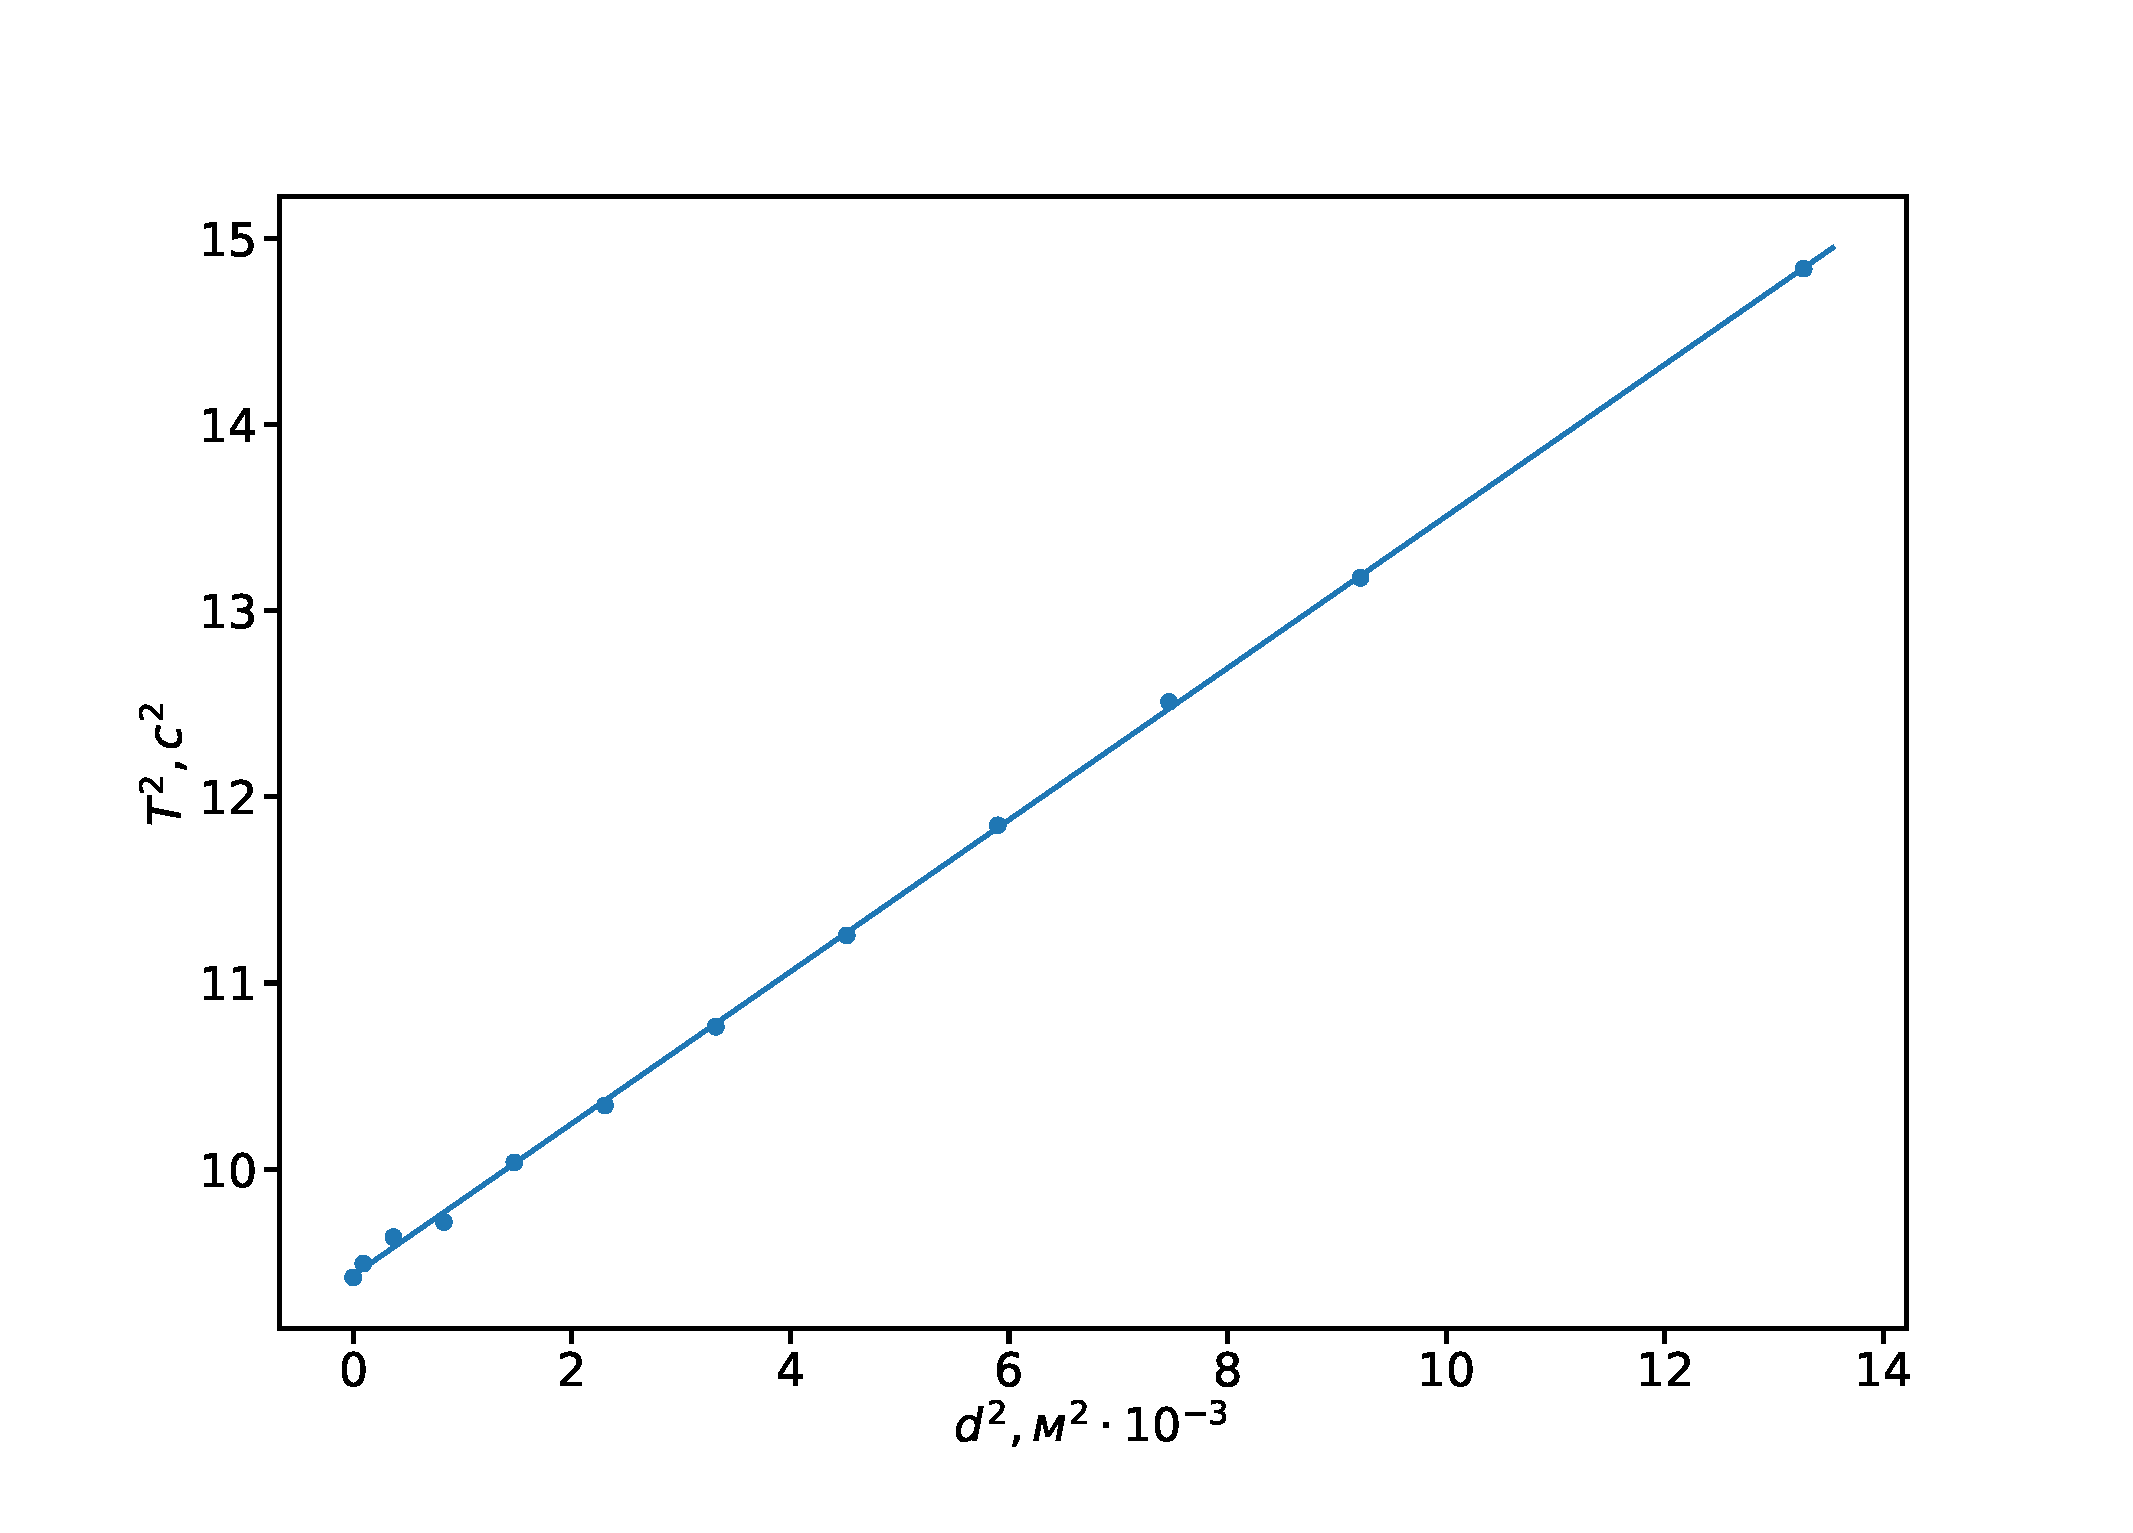
\includegraphics[width=0.8\textwidth]{1.eps}
    \end{center}
    \caption{График зависимости квадрата периода колебаний системы из двух полуциллиндров $T^2$ от квадрата расстояние $h^2$ между их центром масс
    и ценром одного из грузов. Кресты погрешности по оси $T^2$ много меньше масштабов графика и не были нанесены. 
    Кресты погрешности по оси $h^2$ много меньше масштабов графика и не были нанесены.}
    \label{fig:4}
\end{figure}

Из сдвига графика по оси $T^2$ рассчитан момент инерции полуциллиндра $I_{exp} = (8.42 \pm 0.11) \cdot 10^{-4}\textrm{ кг}\cdot\textrm{м}^2$, 
что совпадает с моментом инерции полуциллиндра, рассчитанного теоретически (Прил. \ref{app_3}). Относительная погрешность момента инерции, найденного графически,
равна $\sigma_g = 1\%$, что совпадает с относительной погрешностью одноточечного измерения.

Из совпадения моментов инерции тел, рассчитанных теоретически и экспериментально, можно установить корректность метода. Небольшое увеличение 
относительной погрешности (8 раз) позволяет говорить об эффективности метода измерения момента инерции сложных тел с использованием трифилярного 
подвеса.

\section{Выводы}
Моменты инерции, измереннные с использованием трифилярного подвеса совпали с теоретически предсказанными, из чего может следовать корректность
метода определения моментов инерции тел на трифилярном подвесе. Относительная погрешность полученных результатов составила $1\%$, что в 8 раз 
больше погрешности теоретических рассчитанных моментов инерции.

\section{Использованная литература}
\begin{thebibliography}{9}
    \bibitem{LabBook}
    Лабораторный практикум по общей физике, Том 1, под редакцией А. Д. Гладуна
\end{thebibliography}

\section{Приложения}
\subsection{Теретический расчёт моментов инерции тел} \label{app_1}
Момент инерции полого циллиндра выражается через его массу $m$, внешний и внутренний радиусы $r_1$ и $r_2$:
$$I_1 = \frac{m({r_1}^2 + {r_2}^2)}{2}$$
Момент инерции циллиндрической крышки выражается через радиусы малого и большого циллиндра $r_1$ и $r_2$ и их высоты $h_1$ и $h_2$:
$$I_2 = \frac{m}{2}\left(\frac{{r_1}^4h_1 + {r_2}^4h_2}{{r_1}^2h_1 + {r_2}^2h_2}\right)$$
Момент инерции полуциллиндра радиусом $R$ и массой $m$:
$$I_3 = \frac{mR^2}{4}$$
\subsection{Параметры трифилярного подвеса} \label{app_2}
\begin{table}[H]
    \centering
    \begin{tabular}{|l|l|l|l|l|l|}
        \hline
        $m$, г           & $R$, см         & $r$, см        & $z_0$, м         & $k$, $\frac{\textrm{м}^2}{\textrm{с}^2} \cdot 10^{-4}$ & $I_0, \textrm{ кг}\cdot\textrm{м}^2\cdot 10^{-3}$ \\ 
        \hline
        $1026.4 \pm 0.5$ & $115.5 \pm 0.5$ & $30.2 \pm 0.3$ & $2.158 \pm 0.01$ & $4.01 \pm 0.05$                                        & $8.0 \pm 0.1$                                     \\
        \hline
    \end{tabular}
    
    \caption{Параметры трифилярного подвесса. $m$ - масса диска трифилярного подвеса,
        $R$ - радиус нижнего диска, $r$ - радиус верхнего диска, $z_0$ - расстояние между дисками трифилярного подвеса, $k$ - совокупный 
        параметр системы, $I_0$ - момент инерции трифилярного подвеса}
    \label{tab:1}
\end{table}
\subsection{Параметры измеряемых грузов} \label{app_3}
Первый груз характеризуется внутренним и внешним радиусами $r_1 = 75.2 \pm 0.1$ см и $r_2 = 79.3 \pm 0.1$ см и массой $m = 730.4 \pm 0.1$ г. Рассчитанный момент инерции $I_1 = (4.362 \pm 0.009)\cdot 10^{-3}\textrm{ кг}\cdot\textrm{м}^2$.
Второй груз характеризуется радиусами двух циллиндров $r_1 = 5.2 \pm 0.1$ см и $r_2 = 85.3 \pm 0.1$ см и соответствующими высотами $h_1 = 26.0 \pm 0.1$ см и $h_2 = 3.6 \pm 0.1$ см и массой $m = 584.1 \pm 0.1$ г. 
Рассчитанный момент инерции $I_2 = (2.07 \pm 0.006)\cdot 10^{-3}\textrm{ кг}\cdot\textrm{м}^2$.
Третий груз характеризуется радиусом $r = 45.6 \pm 0.1$ см и массой $m = 763.45 \pm 0.1$ г. Рассчитанный момент инерции $I_3 = (7.94 \pm 0.04) \cdot 10^{-4}\textrm{ кг}\cdot\textrm{м}^2$.
\subsection{Измерения периодов колебаний трифилярного подвеса с грузами} \label{app_4}
Период колебаний 1 груза $T_1 = 4.1860 \pm 0.0005$
Период колебаний 2 груза $T_1 = 3.948 \pm 0.0005$
Период колебаний 1 и 2 грузов вместе $T_{12} = 3.928 \pm 0.0005$
\begin{table}[H]
    \centering
    \begin{tabular}{|l|r|r|r|r|}
        \hline
           & $T$, с   & $h$, м   & $h^2, \textrm{ м}^2$ & $T^2, \textrm{ с}^2$ \\
        \hline
        0  & 3.069000 & 0.000000 & 0.000000             & 9.418761             \\
        1  & 3.081000 & 0.009600 & 0.000092             & 9.492561             \\
        2  & 3.104000 & 0.019200 & 0.000369             & 9.634816             \\
        3  & 3.117000 & 0.028800 & 0.000829             & 9.715689             \\
        4  & 3.168000 & 0.038400 & 0.001475             & 10.036224            \\
        5  & 3.216000 & 0.048000 & 0.002304             & 10.342656            \\
        6  & 3.281000 & 0.057600 & 0.003318             & 10.764961            \\
        7  & 3.355000 & 0.067200 & 0.004516             & 11.256025            \\
        8  & 3.442000 & 0.076800 & 0.005898             & 11.847364            \\
        9  & 3.537000 & 0.086400 & 0.007465             & 12.510369            \\
        10 & 3.630000 & 0.096000 & 0.009216             & 13.176900            \\
        11 & 3.852000 & 0.115200 & 0.013271             & 14.837904            \\
        \hline
    \end{tabular}
    
    \caption{Данные измерения периода колебаний системы $T$ с двумя полуциллиндрами в зависисмости расстояния $h$ до их центров.}
    \label{tab:2}
\end{table}

\end{document}